\section{実装}

本章ではわかるらんどの実装について述べる。

クライアントはブラウザ上のJavaScriptで実装した。

サーバーは並列計算プリミティブLindaをSocket.IO上に実装したlinda-server\footnote{https://github.com/node-linda/linda}を用いて実装している。
Lindaとは1980年代に生まれた並列処理を行うための実装モデルで、
タプルスペース(tuplespace)と呼ばれる共有メモリ空間にデータレコード(タプル)を格納する。
linda-serverを使用することで、各クライアントやデバイス間で直接送信をする処理を記述する必要がなく、
非常に簡潔に拡張性の高い並列処理環境を実現できる。

わかるらんどへの入力はHTTP通信ができる環境であれば可能であるため、Arduino\footnote{https://www.arduino.cc}やRaspberry Pi\footnote{https://www.raspberrypi.org}などで作った各種の入力ハードウェアを利用することができる。
図\ref{button}は「へぇ〜」というスタンプを表示する入力装置である。図\ref{10key}は外付けのテンキーのキーに各種のスタンプの入力を割り当てたものである。
このようにブラウザの投稿画面だけでなく、現状のGUIでは利用されないようなデバイスを作ってわかるらんどの入力装置として利用することができる。

\begin{figure}[h]
\centering
\includegraphics[width=7cm]{images/button.eps}
\caption{「へぇ〜」専用入力装置}
\label{button}
\end{figure}

\begin{figure}[h]
\centering
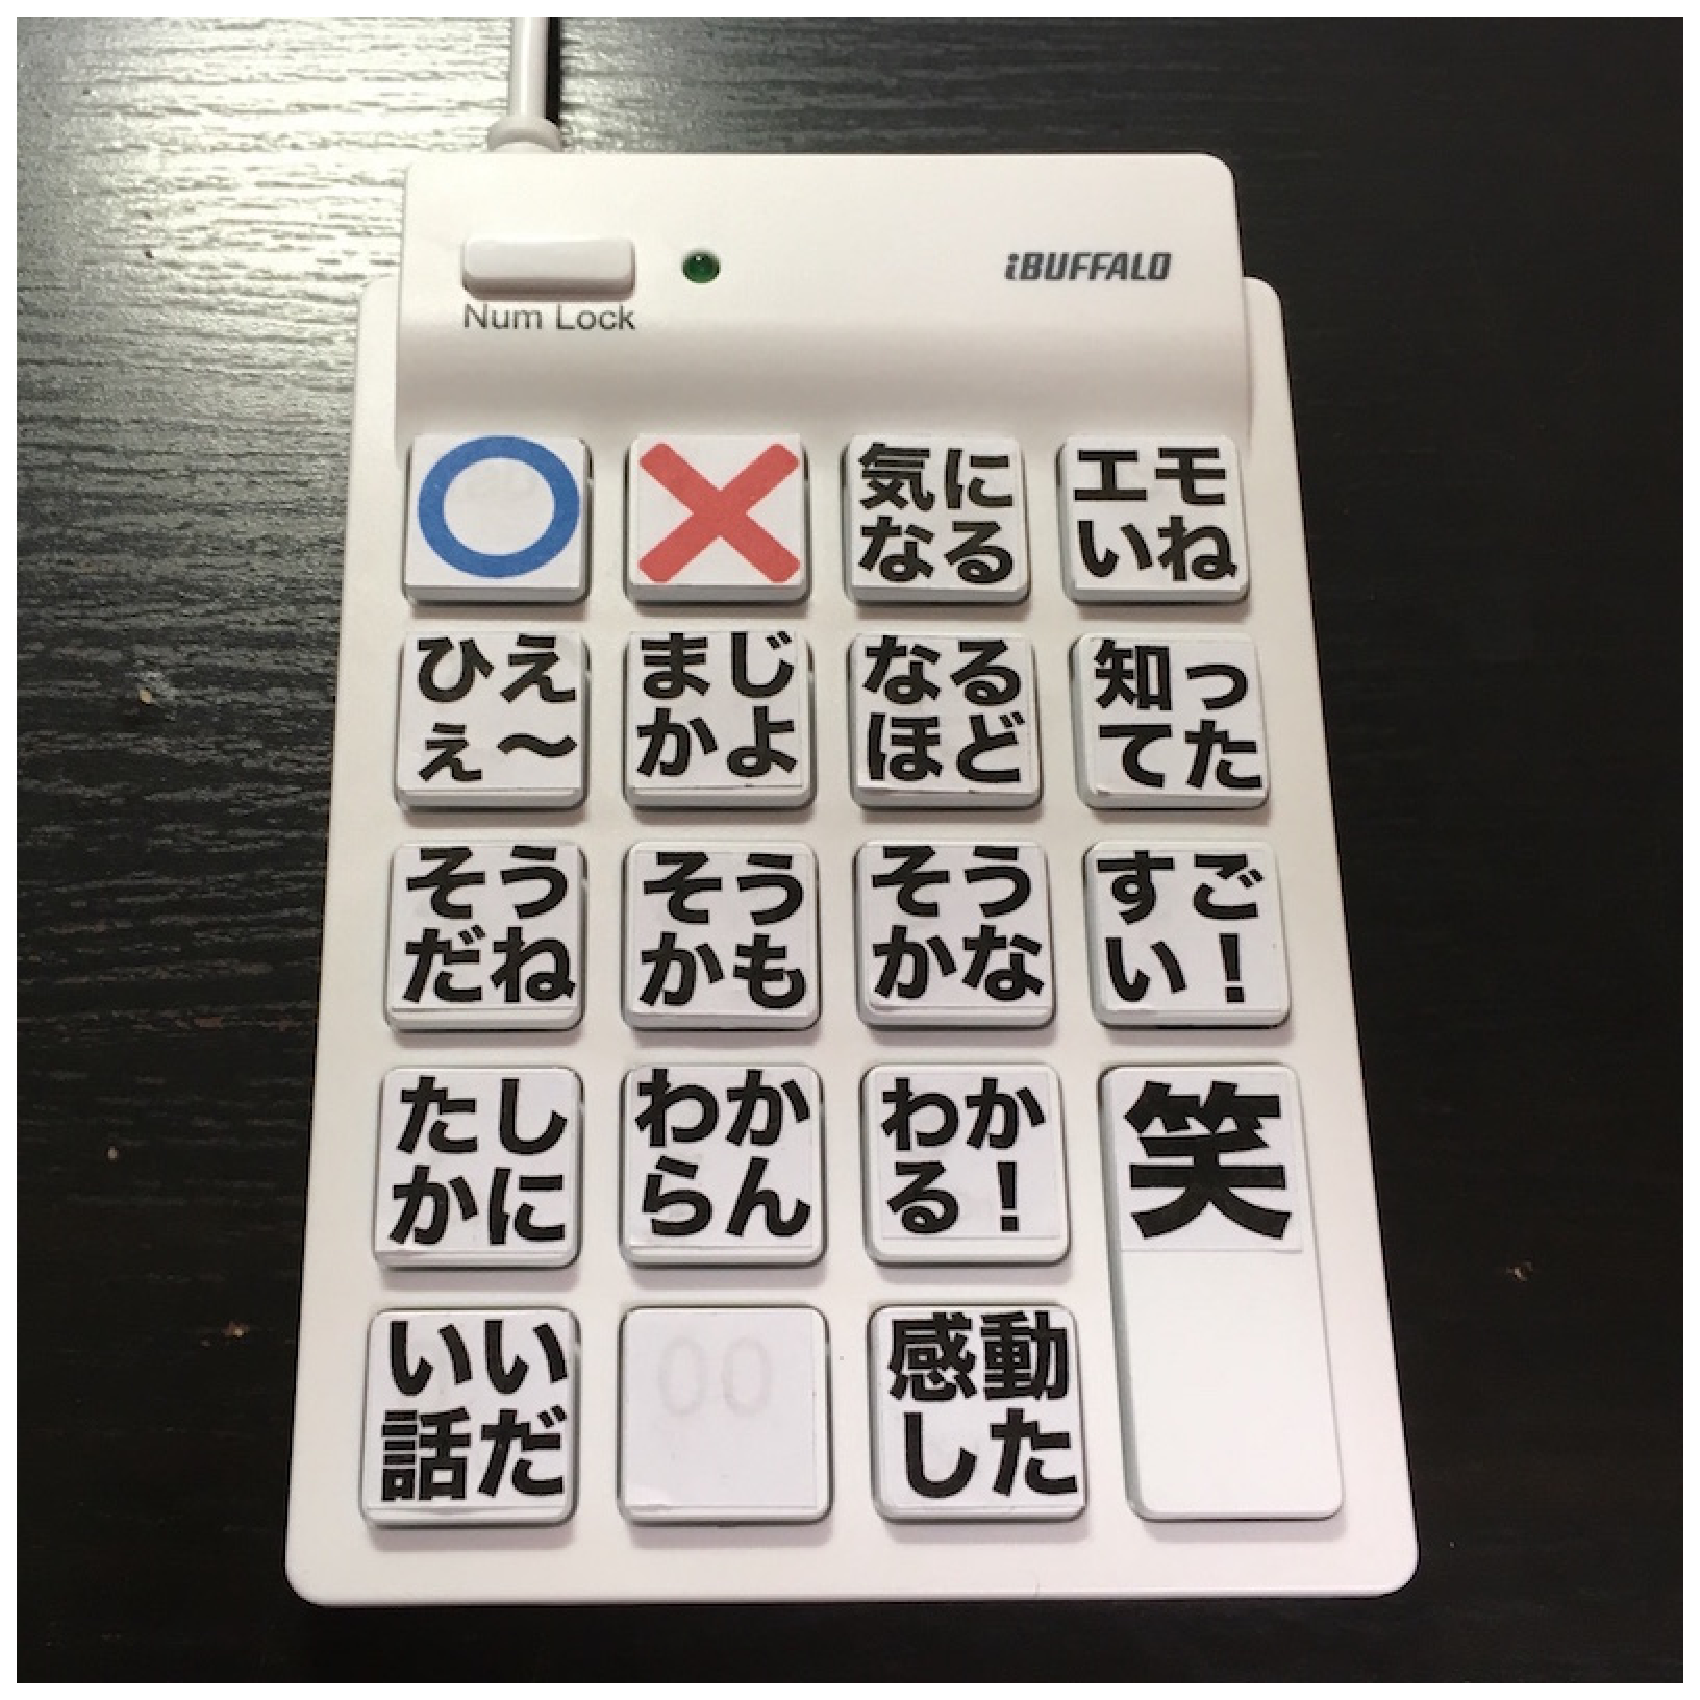
\includegraphics[width=7cm]{images/10key.eps}
\caption{テンキーを利用した入力装置}
\label{10key}
\end{figure}